%!TEX root = /Users/andy/Documents/Academics/Dissertation/thesis.tex

\begin{comment}
	Points to make here:
	Navigatoin is worthy of study
	Omega turn is a critical part of navigation
	
\end{comment}

\chapter{Neural activity of the Omega Turn}\label{chapter:omegaTurn}



\newthought{There has a been frenzy of investigations} by \textit{C. elegans} researchers around the globe to study changes in the neural activity of the motor circuit between  the worm's forward and reverse locomotion [CITE Schafer, Mei Zhen, Lockery, Piggot]. Three of these works were published only in the past few months. In the ongoing work presented here, we study the neural activity that underlies the omega turn, which also includes two such transitions between  forward and reverse locomotion. We confirm some of the results found by others,  clarify certain ambiguities in the literature and use our rich and detailed behavioral readout to probe more deeply at correlations between  neural activity and specific subtle behaviors critical for navigation.


\section{Motivation}

Navigation is a goal directed locomotion, common across species, in which an organism moves toward or away from a cue.  At the neuronal level, navigation requires the temporal coordination of different motor programs.  How does an animal's nervous system orchestrate the changes in locomotion required for navigation? The \textit{Caenorhabditis elegans} escape response provides a platform upon which to investigate how navigation is carried out by a simple nervous system.  

Navigation in  \textit{C. elegans} is regulated by ventrally or dorsally biased head swings (Iino and Yoshida, 2009) and deep ventral omega turns that reorient the worm in the opposite direction.  When the worm is touched on its anterior, it exhibits an escape response by pausing, reversing and turning ventrally in what is often called an omega turn.  The neural circuit for this escape response employs cells at all levels of the nervous system: mechanosensory neurons, command neurons, motor neurons, and muscle. The circuit plays an important role in the animal's decision making, the coordination of its motor programs and its turning behavior. 
The analysis of this stereotyped omega turn provides an opportunity to identify the  neuronal mechanisms that the nervous system employs to translate sensory information into navigational behavior.  


In this chapter we present ongoing work to explore the neural activity underlying the omega turn. A real-time tracking system was developed to record intracellular calcium transients in single neurons while simultaneously monitoring the macroscopic behavior of a freely moving worm as it undergoes an escape response.

[CHECK THE RIM DATA] Importantly, this work lays to rest some confusion in the field about the contribution of the neuron RIM to the escape response.  [TRUE?]

 
\section{Dual-Magnification Calcium and Behavior Imaging}
\subsection{Background}
To study the neural activity of an omega turn requires a system that permits simultaneous observation of neural activity and behavior in freely moving worms.  In particular, it is important to be able to correlate individual neural activity to rich details of the worm's behavior, such as changes in curvature or direction.


Genetically encoded fluorescent calcium indicators such as Cameleon [CITE ME!!!] and GCaMP [CITE ME!] are the primary tools available for optical neurophysiology in \textit{C. elegans}.  The fluorescence of these indicators change with the level of intracellular calcium present. Calcium is often a good indicator of neural activity. As a result, the fluorescent levels can be monitored and neural activity can be inferred.


Calcium imaging is often performed at high magnification (20x or more)  to resolve individual neurons and with high numerical aperture (NA) objectives to collect large numbers of photons. As a result, calcium imaging had traditionally been  performed on immobilized  [ANDY: CITE A SAMUEL LAB PAPER] or partially restrained animals  [ANDY: CITE A SAMUEL LAB PAPER], where it is possible to keep the neurons of interest in a small field of view for an extended period of time. 

The Samuel Lab pioneered the first system to perform calcium imaging in a moving worm \citep{clark_temporal_2007}. In that system, the user manually adjusted a joystick to track the neuron AFD in the head of an unrestrained worm on a motorized stage. The worm was imaged with a high NA 20x objective. This system allowed the user to observe calcium transients in a worm as it moved. However, because the field of view only included a small portion of the worm, details of the worm's behavior like its curvature were not visible.  Additionally, manual tracking made it difficult to consistently track abrupt changes in the worm's  motion.

Since then, a number of groups have developed manual [cite Mei Zhen]  and automated  [cite Shawn lockery, Shafer, pigott]\citep{faumont_image-free_2011}
 tracking systems for calcium imaging in moving worms, using a variety of home built [cite shafer, mei zhen, pigott] and commercial [shawn lockery] systems. 

We have a developed a new tracking system that offers unique advantages. The system is built around a spinning disk confocal microscope which cuts down on background fluorescence and increases signal to noise. The system identifies target neurons from the worm's outline, rather than from their fluorescence which makes it well suited for transgenic animals that exhibit fluorescence in more then one neuron. Additionally, the system builds on our previous experience developing rich behavioral monitors and thus provides high spatiotemporal behavioral data including the worm's instantaneous curvature and orientation.  


\subsection{The DualMag System}
A tracking microscope was built capable of recording calcium transients in a moving worm. The microscope operates at two magnification levels simultaneously, one beam path operates at high-magnification to resolve single neurons, while the other beam path operates at low  magnification to view the entire body of the worm. Real-time computer vision software monitors the position of the body of the worm from the low-magnification beam path and adjusts a motorized stage to keep targeted neurons in the high-magnification field of view. The entire system is called the DualMag.


The DualMag system is built around an upright Nikon [BLAH] microscope body with a spinning disk confocal unit [Andor blah balh and Yokagawa], a motorized stage and an additional low magnification imaging path. See Figure~\ref{fig:omegaSchematic}. 


\begin{figure} %Schematic of DualMag
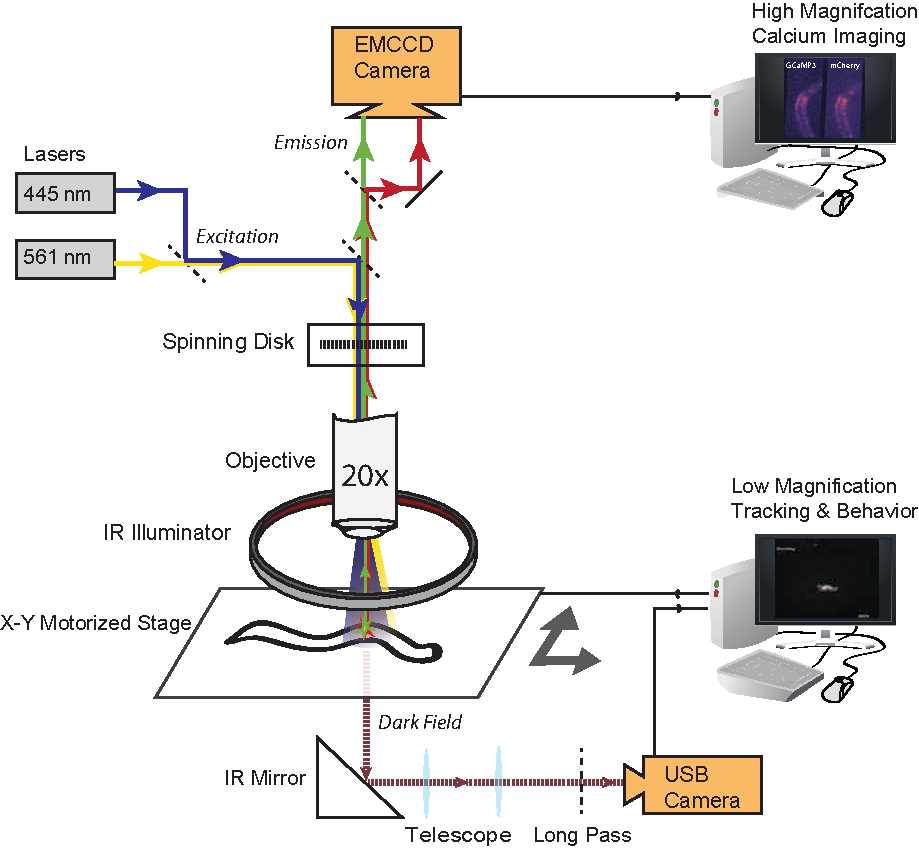
\includegraphics[width=\textwidth]{figures/omegaCalciumImagingSetup}
\caption[DualMag system apparatus.]{Schematic of the DualMag setup, permitting simultaneous recording of intracellular calcium transients and behavior in freely moving \textit{C. elegans}.  A transgenic worm, expressing GCaMP3 and mCherry in targeted neurons, crawls freely on a motorized stage under infrared illumination. An inexpensive USB camera images the worm's motion at low magnification. Real-time computer vision software rapidly analyzes each low magnification image and identifies the location and orientation of the worm and the targeted neuron and adjust the stage to keep the targeted neuron centered beneath a 20x objective used for calcium imaging.  Blue and yellow laser light shine through the 20x objective to excite GCaMp3 and mCherry in the targeted neuron. The emitted green and red fluorescence  is imaged through a spinning-disk confocal microscope onto two halves of an electron multiplying CCD camera.  Comparing the fluorescence in the green and red  channel images gives the relative level of calcium in the neuron. Slanted dashed lines indicate dichroic mirrors. \label{fig:omegaSchematic}}
\end{figure}


A transgenic animal  expressing GCaMP3 and mCherry in targeted neurons crawls freely on agar in a petri dish on a motorized stage under dark field infrared illumination. The high magnification beam path illuminates targeted neurons with  blue (445 nm) and yellow (561 nm) laser light though the spinning-disk confocal system, emitting fluorescence from GCaMP3 in the green and from mCherry in the red. Dichroic mirrors filter out the excitation light and pass only the emitted light to a DualView [CITE] unit which projects the red and green channels side-by-side onto the sensor of an  EMCCD camera. See Figure \ref{fig:omegaSampleImages}c. 


\begin{figure}  %Sample Images of AVB 
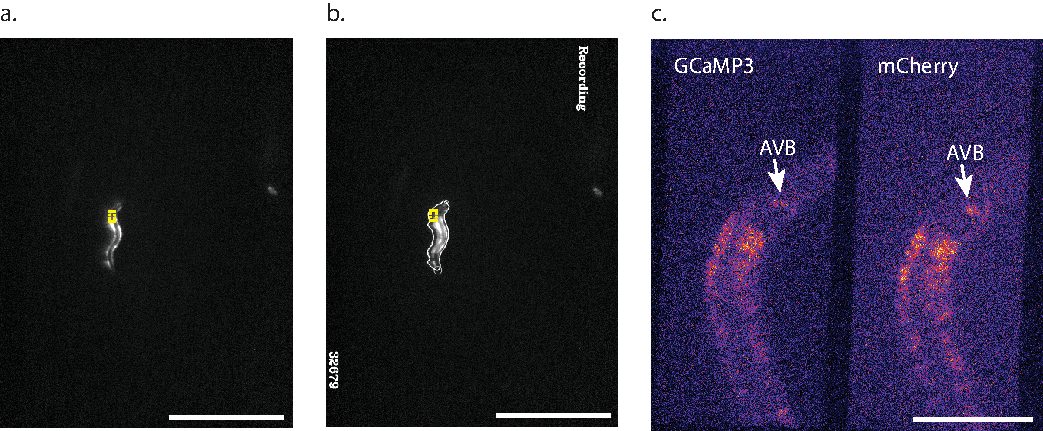
\includegraphics[width=\textwidth]{figures/omegaDualMagImagesWithScale}
\caption[Example images from the DualMag setup.]{Example images of the DualMag setup. Transgenic worm expressing GCaMP3 and mCherry in the AVB interneuron is observed in the DualMag system. \textbf{(a)} Raw-image of worm behavior recorded by the low-magnification beam path is shown. Scale bar is 1mm.  \textbf{(b)} Real-time computer vision software identifies the outline of the worm, its head and tail, and identifies the position of AVB for tracking. Scale bar is 1mm. \textbf{(c)} The high magnification beam path images the yellow square region shown in \textbf{b}. Green channel (left) shows calcium-dependent GCaMP3 fluorescence. Red channel (right) shows calcium-independent mCherry fluorescence. Scale bar is 100 \textmu m.
\label{fig:omegaSampleImages}}
\end{figure}

A second beam path, beneath the microscope images the infrared light scattered by the worm at low magnification. An inexpensive USB CCD camera monitors the worm's position and orientation at 30 fps. See Figure \ref{fig:omegaSampleImages}a. Custom real-time computer vision software written in C identifies the worm's outline, its head and tail,  and the location of targeted neurons (Figure \ref{fig:omegaSampleImages}b) and instructs the motorized stage to adjust its stage velocity to compensate for the worm's motion and to keep the targeted neuron squarely in the center of the high-magnification field of view. The feedback loop operates at 30 Hz and is sufficient to compensate for the worm's movements. See Figures \ref{fig:omegaTimeLapse} and \ref{fig:omegaMontage}.


\begin{figure}  %Time Lapse Image
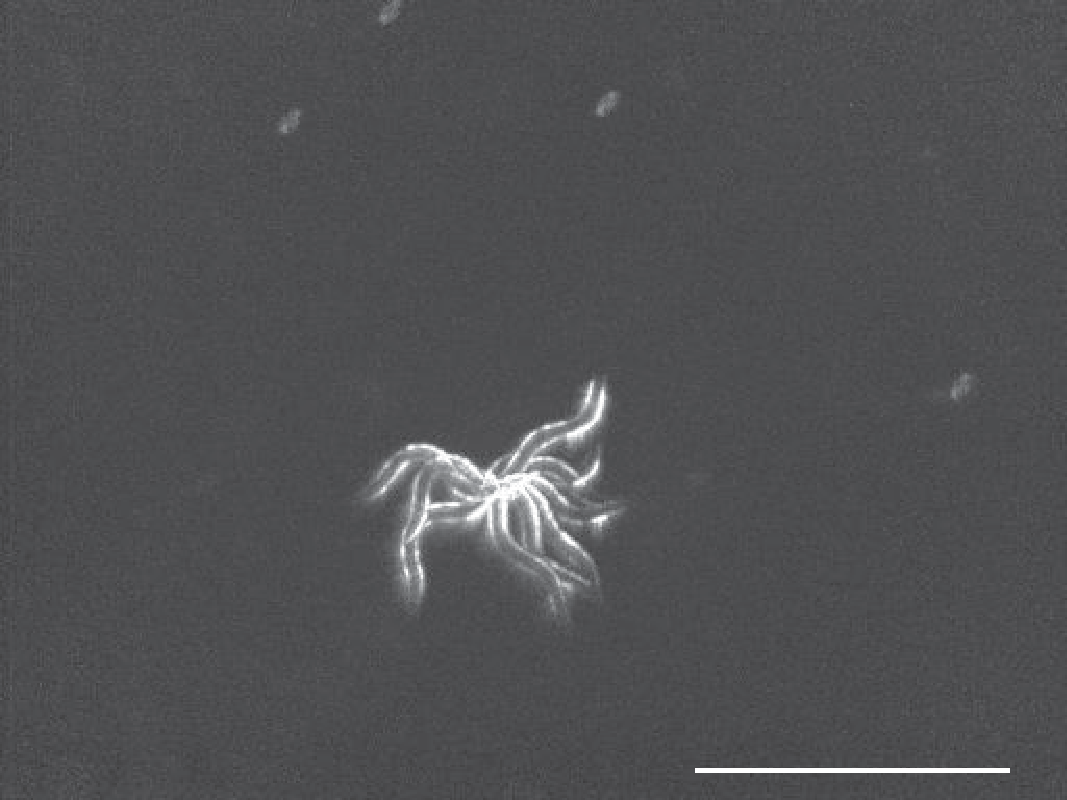
\includegraphics[width=\textwidth]{figures/omegaTimeLapse}
\caption[Time lapse image of behavior from low magnification beam path.]{Time-lapse stroboscopic darkfield image of worm behavior from the low magnification beam path is shown. The DualMag system continually adjusts the stage's velocity to isolate motion in a region of the worm's head. A 28 ms exposure image was taken every 3 seconds for 1 minute. Scale bar is 1 mm.
\label{fig:omegaTimeLapse}}
\end{figure}




While similar in principal to prior work [schaeffer, shawn lockery] this is the first system to our knowledge, that uses a  spinning disk confocal microscope which cuts down on background fluorescence. Second, it uses an inexpensive USB camera to do the tracking and  leverages the real-time computer vision software from the CoLBeRT system \citep{leifer_optogenetic_2011} to perform rapid feedback based on the worm's morphology, not individual neuron fluorescence.













%Montage




\section{Neural Activity of the Escape Response}
The escape response in \textit{C. elegans} can be elicited by gently touching the anterior of the worm. The response is  stereotyped: The worm first ceases its forward locomotion and exploratory head movements (Alkema et al., 2005), it then moves backward away from the stimulus (Chalfie et al., 1985), comes to a stop, and then bends its head ventrally to execute a deep ventral turn before finally reinitiating forward locomotion.  The entire sequence is commonly referred to as an omega turn. 

\begin{figure}  %Montage of an Omega Turn
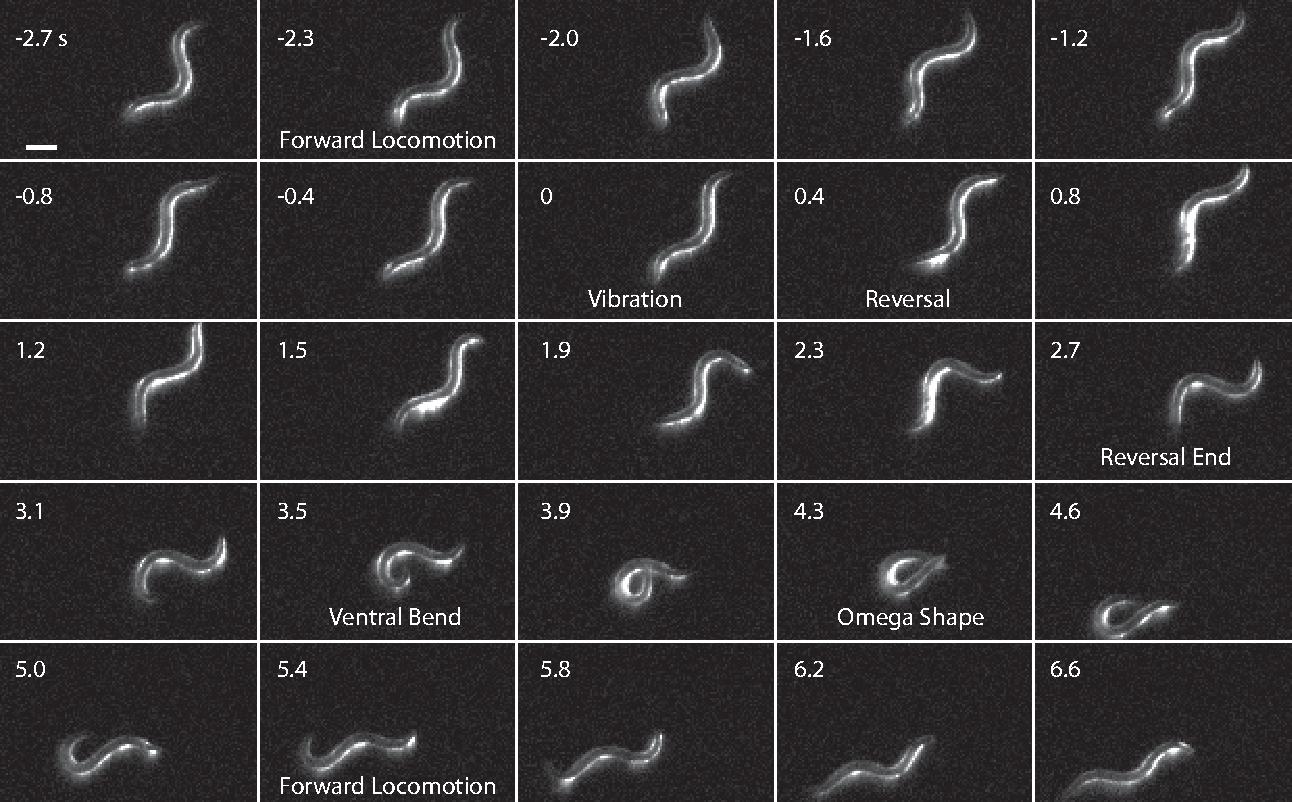
\includegraphics[width=\textwidth]{figures/omegaMontage}
\caption[Video of worm escape response.]{Video of worm escape response is shown. The worm undergoes forward locomotion.  At 0 s, an electric toothbrush vibrates the worm's petri dish and the worm halts forward locomotion and begins a reversal. At 2.7 s the worm ceases reversing and begins a deep ventral bend. At 4.3 s the worm exhibits the omega shape that gives the omega turn its name. At 5.4 s the worm recommences forward locomotion. Scale bar is 100 \textmu m.
\label{fig:omegaMontage}}
\end{figure}



C. elegans crawls on its side in a sinusoidal pattern by propagating dorso-ventral flexures along the anterior-posterior axis of the body.  






 The escape response is initiated by mechanosensory neurons which transduce sensory information through locomotion command neurons to excitatory and inhibitory motor neurons that innervate the body wall muscles (Chalfie et al., 1985)



Gentle touch to the anterior of the worm induces an escape response where the animal stops exploratory head movements (Alkema et al., 2005) and moves backward away from the stimulus (Chalfie et al., 1985).  The escape response is initiated by mechanosensory neurons which transduce sensory information through locomotion command neurons to excitatory and inhibitory motor neurons that innervate the body wall muscles (Chalfie et al., 1985).  Reinitiation of forward locomotion is accompanied by a steep ventral head bend followed by a deep turn (omega turn) that redirects the worm away from the stimulus.  

The analysis of the worm escape response gives us the  opportunity to identify the molecular and neuronal mechanisms  the nervous system employs to translate sensory information into navigational behavior. 

Genetically encoded calcium indicators in combination with  computer vision worm tracking will be used to determine the activity patterns of mechanosensory neurons, locomotion command neurons, neck motor neurons and neck muscles during turning behavior.  

Unraveling the neural circuitry required for turning behavior will lead to the understanding of the neural and molecular machinery that confers flexibility in the output of coordinated motor programs.



\section{Methods}


\subsection{Calcium Imaging in Moving Worm}
\subsubsection{Optics}

Blue (445 nm) and yellow (561 nm) lasers are fiber-coupled into the spinning disk system. Using a 20x objective with a field of view  about 300 \textmu m wide, each laser  provides a maximum power output of 20mW/mm$^2$. An Andor Ion BLAH BLAH BLAH camera images fluorescence at 20Hz with an exposure time of 50ms. 

The condensor lens was removed from the bottom of the microscope to make room for a second low-magnifcation beam path. A an IR prism mirror reflects infrared light into an optical train composed of a telescope and a long pass filter.  

In the experiments described here, the blue laser was run at 3 mW/mm$^2$ and the yellow laser was run at 10 mW/mm$^2$ to avoid pohotobleaching. 

Custom made infrared illumination ring of 100 LED's at 850 nm. 
Thorlabs FEL0750  750nm Longpass Filter.





\subsubsection{Real-Time Tracking}
MAC 6000 [ANDY GRAB ALL OF THIS FROM THE COLBERT SYSTEM] connected over USB, running Windows XP. 
Imaging Source Camera [ANDY Look it up.]
Modified version of the MindControl software, written in C using OpenCV open source computer vision library with hardware optimized Intel Integrated Performance Primitives [ANDY cite other chapter]. 

In brief:
Identifies the outline of the worm, finds the head tail, segments the worm into coordinates, then identifies the targeted neuron within the coordinate system. Finally, the software measures the distance of the targeted neuron from the center of the high magnification field of view and adjusts the stage velocity to glide the worm back towards the center. 

[ANDY CLEAN UP HERE]


The software is essentially the same as in [CITE BEFORE] with the following minor modifications, which were necessary to address poor lighting and the demands for more rapid tracking: When identifying the outline of the worm the software now performs a dilation on the image [CITE LEARNING OPENCV] which can compensate for ``holes'' that appear in the worm due to imaging through the agar plate. The newer version also allows the the outline of the worm to be smoothed directly, wheras the old version only allowed the underlying image to be smoothed. Finally the new version of the software provides finer control of the stage response to the feedback loop. 




\subsubsection{Video Synchronization}
The DualMag system records two independent video streams recorded at different frame rates on different computers. The two video streams are synchronized by shining synchronous pulses of LED light at the appropriate wavelength into both cameras. LEDs are controlled independently from the other software mentioned by a custom LabView program  interfaced with a LabJack digital to analog converter. [BLAH BLAH BLAH. ANDY Find LABJACK] The flashes of light are identified manually offline during post processing. 

\subsubsection{Video Analysis}





\section{Manuscript Information}
The work presented here was done by Andrew M. Leifer in close collaboration with Christopher Clark and Mark Alkema of the Alkema Lab. Andrew Leifer built the hardware with Mason Klein. Christopher Clark and Andrew Leifer together performed all of the experiments. Christopher generated the worm strains. Andrew wrote all software and analyzed the data. Both Andrew and Christopher wrote the manuscript. Lauren Freeman built the video synchronization LED system. 






Animals navigate their environment to locate favorable conditions, find food, find a mate and avoid predation. While principles of basic locomotion for many animals including humans are well understood, little is known about the molecular and neural mechanisms of goal directed locomotion.  Navigation requires the integration of various sensory stimuli followed by precise orchestration of musculature to produce goal directed movement.  Animals ranging from fruit flies to humans integrate visual, olfactory, and mechanical sensory inputs to determine their current and desired locations.  How does an animal process sensory information to navigate its environment?  Defining sensorimotor circuits requires not only a detailed knowledge of the neural connectivity of the nervous system, but also the ability to manipulate the functions of the component neurons. The simplicity and completely defined synaptic connectivity of the nervous system of the nematode C. elegans provides a unique opportunity to fully define the cellular and molecular pathways which regulate navigational behavior.

Navigation is a goal directed locomotion in which an animal must generate asymmetry in their locomotion program to steer toward or away from a cue.  At the neuronal level, navigation requires the temporal coordination of different motor programs.  How does an animal generate asymmetry in a locomotion program allowing it to steer and change direction?  C. elegans navigation is regulated by ventrally or dorsally biased head swings (Iino and Yoshida, 2009) and deep ventral omega turns that reorient the worm in the opposite direction.  The neural circuit for the C. elegans escape response provides a paradigm to investigate how an animal changes direction.  This circuit employs mechanosensory neurons, command neurons and motor neurons to govern decision making, the coordination of motor programs and turning behavior. C. elegans crawls on its side in a sinusoidal pattern by propagating dorso-ventral flexures along the anterior-posterior axis of the body.  Gentle touch to the anterior of the worm induces an escape response where the animal stops exploratory head movements (Alkema et al., 2005) and moves backward away from the stimulus (Chalfie et al., 1985).  The escape response is initiated by mechanosensory neurons which transduce sensory information through locomotion command neurons to excitatory and inhibitory motor neurons that innervate the body wall muscles (Chalfie et al., 1985).  Reinitiation of forward locomotion is accompanied by a steep ventral head bend followed by a deep turn (omega turn) that redirects the worm away from the stimulus.  The analysis of the worm escape response gives us the unique opportunity to identify the molecular and neuronal mechanisms of how the nervous system translates sensory information into navigational behavior. Genetically encoded calcium indicators in combination with machine-vision worm tracking will be used to determine the activity patterns of mechanosensory neurons, locomotion command neurons, neck motor neurons and neck muscles during turning behavior.  Unraveling the neural circuitry required for turning behavior will lead to the understanding of the neural and molecular machinery that confers flexibility in the output of coordinated motor programs.

I will express the fluorescent calcium sensor, GCaMP3 (Tian et al., 2009), in the AVM and ALM mechanosensory neurons, the AVA and AVB locomotion command neurons; the RMD, SMD and RIV neck motor neurons; and muscles with the mec-4, rig-3, lgc-55, lim-4 and myo-3 promoters (Sagasti et al., 1999; Pirri et al., 2009; Brockie et al., 2001; Ardizzi and Epstein, 1987).  With these transgenic lines, I will analyze mechanosensory neuron, command neuron, motor neuron and neck muscle flourescence to determine their activity during turning behavior.

\begin{comment}
Alkema, M.J., Hunter-Ensor M., Ringstad N. and Horvitz H.R. (2005). Tyramine functions independently of octopamine in the Caenorhabditis elegans nervous system. Neuron 46, 247- 260.

Ardizzi J.P. and Epstein, H.E. (1987). Immunochemical Localization of Myosin Heavy Chain Isoforms and Paramyosin in Developmentally and Structurally Diverse Muscle Cell Types of the Nematode Caenorhabditis elegans. Journal of Cell Biology 105, 2763-2770.

Brockie, P.J., Madsen, D.M., Zheng, Y., Mellem, J. and Maricq A.V. (2001). Differential expression of glutamate receptor subunits in the nervous system of Caenorhabditis elegans and their regulation by the homeodomain protein UNC-42. Journal of Neuroscience 21, 1510-1522.

Chalfie, M., Sulston, J.E., White, J.G., Southgate, E., Thomson, J.N. and Brenner, S. (1985). The Neural Circuit for Touch Sensitivity in Caenorhabditis elegans. Journal of Neuroscience 5, 956-964.

Gray, J.M., Hill, J.J. and Bargmann C.I. (2005). A circuit for navigation in Caenorhabditis elegans. Proceedings of the National Academy of Sciences of the USA 102, 3184-3191.

Iino, Y. and Yoshida, K. (2009). Parallel use of two behavioral mechanisms for chemotaxis in Caenorhabditis elegans. Journal of Neuroscience 29, 5370-5380.

Pirri, J.K., McPherson, A.D., Donnelly, J.L., Francis, M.M. and Alkema, M.J. (2009) A tyramine-gated chloride channel coordinates distinct motor programs of a Caenorhabditis elegans escape
response. Neuron 62, 526-538.

Sagasti, A., Hobert, O., Troemel, E.R., Ruvkun, G. and Bargmann, C.I. (1999). Alternative olfactory neuron fates are specified by the LIM homeobox gene lim-4. Genes \&  Development. 13, 1794- 1806.

Tian, L., Hires, S.A., Mao, T., Huber, D., Chiappe, M.E., Chalasani, S.H., Petreanu, L., Akerboom, J., McKinney, S.A., Schreiter, E.R., Bargmann, C.I., Jayaraman, V., Svoboda, K. and Looger, L.L. (2009). Imaging neural activity in worms, flies and mice with improved GCaMP calcium indicators. Nature Methods 6, 875-881.
\end{comment}
